\chapter{Projekt}
\section{Architektura}
Architektura rozwiązania. Aplikacja stworzona będzie w architekturze klient-serwer. Interfejs użytkownika zrealizowany będzie w technolgii aplikacji internetowych, tak by dostęp do repozytorium nie wymagał instalacji i był dostępny na wszystie platformy. Dodatkowo stworzona zostanie usługa internetowa ( ang. web service ), tak by umożliwić zintegorowanie aplikacji z zewnętrznymi aplikacjami dzięki czemu możliwa będzie automatyzacja kluczowych procesów. Perzystencja danych dokonywana będzie w relacyjnej bazie danych poprzez moduł odwzorowujący obiektową architekturę systemu informatycznego na bazę danych.
\begin{figure}[h]
\centerline{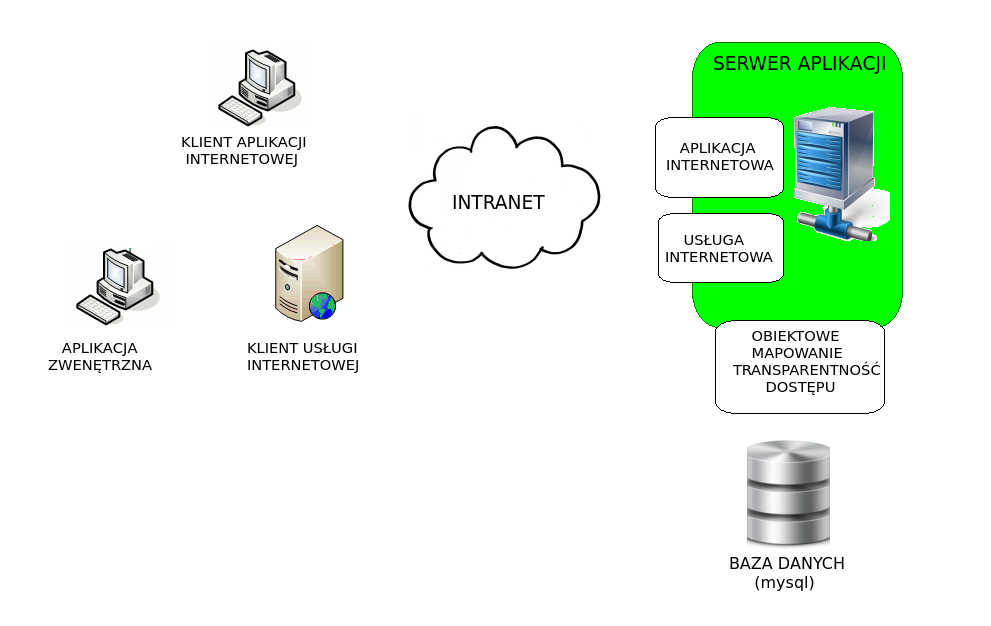
\includegraphics[scale=0.5]{img/architektura.png}}
\caption{Architektura systemu}
\label{fig:architektura}
\end{figure}
\section{Komponenty}
\begin{figure}[h]
\centerline{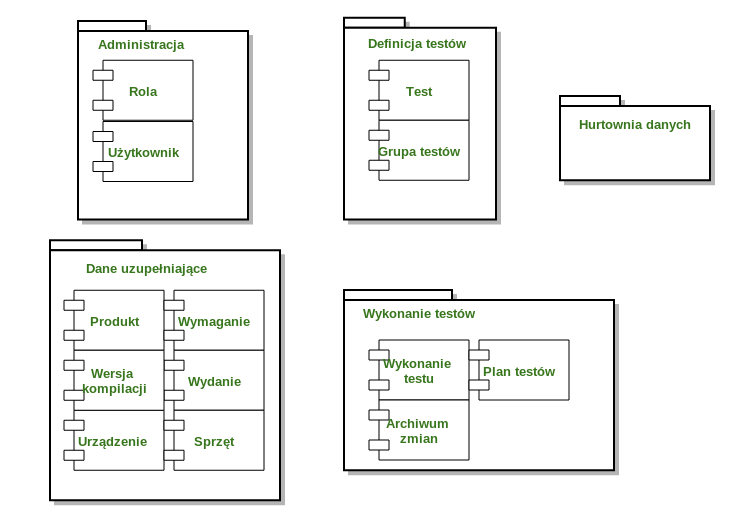
\includegraphics[scale=0.5]{img/komponenty.png}}
\caption{Komponenty systemu}
\label{fig:architektura}
\end{figure}
%<< Diagram fizyczny >>

%<< Diagram komponentów >>

%Komponent zarządzanie użytkownikami

%Komponent Definicji 

%Komponent wykonania testów

%Komponent danych dodatkwych
\section{Warstwy}
\subsection{Warstwa aplikacji internetowej}
Lorem ipsum, lorem ipsum Lorem ipsum, lorem ipsum Lorem ipsum, lorem ipsum Lorem ipsum, lorem ipsum Lorem ipsum, lorem ipsum


\subsection{Warstwa aplikacji internetowej}
Usługa internetowa pozwala na wykonanie trzech akcji:
\begin{enumerate}
  \item dodania wymagań, tak by w ten sposób móc zautomatyzować ten proces, na przykład dodając wprost z zewnętrzej bazy dedykowanej do przechowywania i śledzenia wymagań
  \item pobrania wykonania przypadków testowych dla użytkownika
  \item aktualizacji wykonania przypadku testowego. Udostępnienie dwóch powyższych podpunków pozwala na stworzenie osobnego modułu klienckiego
\end{enumerate}.

\section{Użytkowicy i ich role}

\begin{enumerate}
  \item Obsługa techniczna jest przypisana do poszczególnych planów testowych. Jego zadaniem jest oznaczanie poszczególnych części systemu jako gotowe do użytku. Administrator zajmuje się fizycznym sprzętem jak też instalacją wymaganego oprogramowania
  \item Tester wykonuje przypisane do niego przypadki testowe. Tester wybiera pracę z listy możliwych zadań jak również może mieć z góry przypisane zadania
  \item Lider testów wspiera zespół w wykonywaniu pracy, służy swoją wiedzą i doświadczeniem pomagając podczas napotkania problemów. Lider może również przypisywać testy do poszczególnych testerów jak i wywłaszczać od już przypisanych.
  \item Administrator odpowiedzialny jest za zarządzanie uprawnieniami użytkowników. Przypisuje uprawnienia, tworzy i autoryzuje użytkowików
  \item Pośrednik ( ang. liason ) Odpowiedzialny jest za komunikacje zespołu testów z zespołem programistycznym. Posiaga wgląd do aktulnie wykonywanyh testów i konfiguracji. Jego zadaniem jest rozwiązywanie problemów związanych z jego macierzystym produktem. Pośrednik proponuje również tymczasowe rozwiązania które pozwalają obejść problemy wynikające z błędów w oprogramowaniu, które naprawione będą dopiero podczas przyszłych inkrementów.
  \item
  

\end{enumerate}

\section{Składowe aplikacji}


Podstawową jednostą aplikacji jest przypadek testowy. Składa się on z :
\begin{enumerate}
  \item wymagana konfiguracja, warunków wejściowych
  \item scenariusz, to jest lista kroków do wykonania wraz z oczekiwanymi rezultatami
  \item wymagania które są weryfikowane 
  \item opis
  \item tytuł
  \item identyfikator
  \item estymowany czas potrzebny do wykonaniu
  \item lista urządzeń wymaganych do testów
  \item lista oprogramowania wymaganego do testów
  
\end{enumerate}



Przypadki testowe wchodzą w skład grup testów. Hierarchia ta ma drzewiastą strukturę co oznacza iż grupy mogą być zagnieżdżane. Grupy powinny agregować testy które posiadają podobną charakterystykę. Na przykład testują te same funkcjonalności, wymagają podobnej konfiguracji, urządzeń, dokumentacji. Testy funkcjonalne i niefunkcjonalne nie powinny znajdować się w tym samym przypadku testowym Składowe:
\begin{enumerate}
  \item  tytuł
  \item identyfikator
  \item identyfikator rodzica
\end{enumerate}
 



\chapter{Implementacja}
Interfejs użytkownika stworzony został w technologi aplikacji internetowych przy użyciu technologii Java Server Faces która realizuje wzorzec projektowy  Model-Widok-Kontroler. Warstwa serwerowa działa na serwerze aplikacji Glassfish. Silnik bazodanowy to Mysql, silnik ten może być zmieniony podczas wdrożenia aplikacji poprzez zastosowanie tranparentności dostępu do danych. Moduł odwzorowujący obiektową architekturę systemu informatycznego na bazę danych udostępnia wiele implementacji baz danych przy czym interfejs jest wspólny.

%Dodatkową warstwą dostępu jest dostęp poprzez technologię Web Service REST. Z tego poziomu dostępna jest tylko część funkcjonalnośći. Głównym zastosowaniem dostępu poprzez Web Service jest możliwość zintegrowania aplikacji z zewnętrznymi usługami.Usługa internetowa pozwala na wykonanie trzech akcji:
%- dodania wymagań, tak by w ten sposób móc zautomatyzować ten proces, na przykład dodając wprost z zewnętrzej bazy dedykowanej do przechowywania i śledzenia wymagań
%- pobrania wykonania przypadków testowych dla użytkownika
%- aktualizacji wykonania przypadku testowego. Udostępnienie dwóch powyższych podpunków pozwala na stworzenie osobnego modułu klienckiego


\section{Workflow}
\begin{enumerate}
  \item Tworzony jest nowy projekt
  \item Tworzone są wymagania
  \item Na podstawie wymagań tworzone są grupy testów i przypadki testowe. Scenariusze przypadków testowych tworzone są przy współpracy z zespołem programistycznym.
  \item Tworzony jest nowy plan testów który testować będzie nowe wydanie produktu. Tworzony jest harmonogram uwzlględniający poszczególne inkrementy produktu i testowane funkcjonalności.
  \item Do planu testów dodawane są testy. Podczas dodawania testów należy wziąć pod uwagę pokrycie nowych funkcjonalności i równomierne rozplanowanie testów dla różnych urządzeń.

\end{enumerate}
